\section{Mengenlehre}
\subsection*{Teilmenge und Obermenge}
Wenn $A$ Teilmenge von $B$ ist, dann ist $B$ die Obermenge von $A$ ($B\subseteq A\Leftrightarrow\forall x:x\in B\Rightarrow x\in A$).
Eine Menge $B$ heisst echte Teilmenge von $A$ ($B\subset A$), falls gilt $B\subseteq A\wedge B\neq A$\\

Natürlichen Zahlen $\mathbb{N}_0$ := \{0,1,2,3,4.....\}\\
Ganzen Zahlen  $\mathbb{Z}$ := \{...-3,-2,-1,0,1,2,3,...\}\\
Rationalen Zahlen  $\mathbb{Q}$ := \{...,-0.2,...5...,1.75,...\}\\
Reellen Zahlen   $\mathbb{R}$ := \{...,2.78345..,5,..,$\sqrt{2}$,... \}\\

Für alle Mengen gilt:\\ 
\varnothing \subseteq der\ Menge\ UND\ die\ Menge\ \subseteq der\ Menge\ selbst.\\

\subsection{Mengenoperationen} 
Gegeben sei die Grundmenge G, G := \{Apfel, Birne, Banane, Kiwi, Mango\} und die Teilmengen A und B.
$A$ := \{Apfel, Birne\} B := \{Birne, Banane\}
\fbox{\parbox{\columnwidth}{
\textbf{Vereinigung, Mengenkonjunktion $\cup$} \\ 
$A$ \cup B := \{Apfel, Birne, Banane\} \\
$A$ \cup B := \{x \in G \mid x \in A \vee x \in B\}

\textbf{Durchschnitt, Mengen-Disjunktion} $\cap$\\
$A$ \cap B := \{Birne\} \\ 
$A$ \cap B := \{x \in G \mid x \in A \wedge x \in B\}

\textbf{Differenz} $\setminus$\\
$A$ \setminus B := \{Apfel\} \\ 
$A$ \setminus B := \{x \in G \mid x \in A \wedge x \notin B\}

\textbf{Symmetrische Differenz} $\triangle$\\
$A$ \triangle B := {Apfel, Banane} \\
$A$ \triangle B := \{x \in G \mid (x \in A \wedge x \notin B) \vee(x \in B \wedge x \notin A)\}

\textbf{Komplement} $A^\mathrm{C}$ oder $\overline{\rm A}\\
$A$ ^\mathrm{C} := {Banane,Kiwi,Mango} = A ^\mathrm{C} := \{ x \in G \mid x \notin A \}
}}

\subsection{Hassediagramm}
\begin{wrapfigure}[9]{r}{.46\linewidth}
\vspace{-20pt}
\hspace{-0pt}
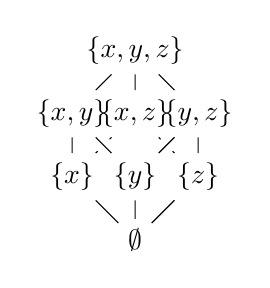
\begin{tikzpicture}[scale=0.4]
  \node (max) at (0,4) {$\{x,y,z\}$};
  \node (a) at (-2,2) {$\{x,y\}$};
  \node (b) at (0,2) {$\{x,z\}$};
  \node (c) at (2,2) {$\{y,z\}$};
  \node (d) at (-2,0) {$\{x\}$};
  \node (e) at (0,0) {$\{y\}$};
  \node (f) at (2,0) {$\{z\}$};
  \node (min) at (0,-2) {$\emptyset$};
  \draw (min) -- (d) -- (a) -- (max) -- (b) -- (f)
  (e) -- (min) -- (f) -- (c) -- (max)
  (d) -- (b);
  \draw[preaction={draw=white, -,line width=6pt}] (a) -- (e) -- (c);
\end{tikzpicture}
\end{wrapfigure}
Man kann die Inklusionsbeziehungen aller Teilmengen in Form eines Hasse-Diagramms veranschaulichen. Das Hasse-Diagramm für $\mathcal{P}(\{x,y,z\})$ lässt sich dann wie folgt darstellen:

\subsection{Venn-Diagramm}
\begin{tikzpicture}[scale=.45]
    \begin{scope}
        \clip \firstcircle;
        \fill[filled] \secondcircle;
    \end{scope}
    \draw[outline] \firstcircle node {$A$};
    \draw[outline] \secondcircle node {$B$};
    \node[anchor=south] at (current bounding box.north) {$A \cap B$};
\end{tikzpicture}
%Set A or B but not (A and B) also known a A xor B
\begin{tikzpicture}[scale=.45]
\hspace{-.5cm}
    \draw[filled, even odd rule] \firstcircle node {$A$}
                                 \secondcircle node{$B$};
    \node[anchor=south] at (current bounding box.north) {$A\triangle B$};
\end{tikzpicture}
% Set A or B
\begin{tikzpicture}[scale=.45]
    \draw[filled] \firstcircle node {$A$}
                  \secondcircle node {$B$};
    \node[anchor=south] at (current bounding box.north) {$A \cup B$};
\end{tikzpicture}
% Set A but not B
\hspace{.5cm}
\begin{tikzpicture}[scale=.45]
    \begin{scope}
        \clip \firstcircle;
        \draw[filled, even odd rule] \firstcircle node {$A$}
                                     \secondcircle;
    \end{scope}
    \draw[outline] \firstcircle
                   \secondcircle node {$B$};
    \node[anchor=south] at (current bounding box.north) {$A\setminus B$};
\end{tikzpicture}

\begin{tikzpicture}[scale=.45]
    \begin{scope}
        \clip \firstcircle;
        \draw[outline] \firstcircle node {$A$}
                                     \secondcircle;
    \end{scope}
    \draw[outline] \firstcircle
                   \secondcircle node {$B$};
    \node[anchor=south] at (current bounding box.north) {$A ^\mathrm{C}$};
\end{tikzpicture}

\subsection{Kartesisches Produkt}
Seien $A,B$ Mengen, dann ist das kartesische Produkt (Kreuzprodukt)
von $A$ und $B$ definiert als: $A\times B:=\{(a,b)\mid a\in A\wedge b\in B\}$. 
$A\times B$ ist die Menge aller geordneten Paare von $A$ und $B$.\\
\emph{Beispiel:}\\
$\{1,2\}\times\{3,4\}=\{(1,3),(1,4),(2,3),(2,4)\}$\\
$\{3,4\}\times\{1,2\}=\{(3,1),(3,2),(4,1),(4,2)\}$\\
-Das Kartesische Produkt ist \textbf{nicht kommutativ}:\\
$A$\times$B$\neq$B$\times$A\\
-Es ist \textbf{nicht assoziativ}:\\
A$\times$(B$\times$C)$\neq$(A$\times$B)$\times$C\\
-Es ist \textbf{indistributiv}:\\
(A$\cup$B)$\times$(C$\cup$D)$\neq$(A$\times$C)$\cup$(B$\times$D)\\
-Leere Mengen:\\
$A\times\emptyset=\emptyset\times A=\emptyset$

\subsection{Elementare Rechenregeln für Mengen}
\fbox{\parbox{\columnwidth}{
\textbf{Assoziativgesetze}\\
$(A\cup B)\cup C=A\cup (B\cup C)$\\
$(A\cap B)\cap C=A\cap (B\cap C)$\\
\textbf{Kommutativgesetze}\\
$A\cup B=B\cup A$\\
$A\cap B=B\cap A$\\
\textbf{Distributivgesetze}\\
$(A\cup B)\cap C=(A\cap C)\cup (B\cap C)$\\
$(A\cap B)\cup C=(A\cup C)\cap (B\cup C)$\\
\textbf{Absorptionsgesetze}\\
$A\cap (A\cup B)=A$\\
$A\cup (A\cap B)=A$\\
\textbf{Idempotenzgesetze}\\
$A\cap A=A$\\
$A\cup A=A$\\
\textbf{Komplementgesetze}($G$ ist Grundmenge)\\
$A\cap\bar{A}=\emptyset$\\
$A\cup\bar{A}=G$\\
\textbf{Identitätsgesetz}\\
$A\cap$G = A && A$\cup$ $\emptyset$=A$\\
 $A\cap$$\emptyset$=$\emptyset$ & A$\cup$G = G\\
  \textbf{De Morgan Gesetz}\\
$(A$\cap$B)^\mathrm{C}$= $A^\mathrm{C}$\cup$ $B^\mathrm{C}$\\ 
(A$\cup$B)^\mathrm{C}$ = $A^\mathrm{C}$\cap$ B^\mathrm{C}$\\
 \textbf{Komplementgesetze}\\
$A$\cap$ $A^\mathrm{C}$ =$\emptyset$ & A$\cup$ $A^\mathrm{C}$ = G\\
($A^\mathrm{C}$)^$\mathrm{C}$ =$\emptyset$ & A $\cup$ $A^\mathrm{C}$ = G\\
$G^\mathrm{C}$ = $\emptyset$&\\
$\{\}^\mathrm{C}$=G &\\
\textbf{Teilmengenbeziehungen}\\
$A$ $\subseteq$B $\Rightarrow$(A$\cap$B=A)& A$\subseteq$B$\Rightarrow$(A$\cup$B =B)\\
 (A$\subseteq$B)$\land$(B$\subseteq$C)$\Rightarrow$(A$\subseteq$C)\\
 Transitivität der Teilmengenbeziehung\\
}}

\subsection{Mächtigkeit, Kardinalität} 
Anzahl Elemente in jener Menge enthalten sind. $\vert$M$\vert$ oder \#M .
Menge unendlich = Kardinalität undendlich. \vert$M$\vert$ := $\infty$ 
\\ 
\subsection{Potenzmengen und deren Kardinalität} 
Die Potenzmenge einer Menge F st die Menge aller Teilmengen.\\
$\mathcal{P}(\{a,b\})=\{\emptyset,\{a\},\{b\},\{a,b\}\}$\\
$\mathcal{P}(\emptyset)=\{\emptyset\}$\\
$\mathcal{P}(\{\emptyset\})=\{\emptyset,\{\emptyset\}\}$\\
$\mathcal{P}(\mathcal{P}(\mathcal{P}(\emptyset)))=\{\emptyset,\{\emptyset\},\{\{\emptyset\}\},\{\emptyset,\{\emptyset\}\}\}$

Ein Mengensystem von F ist eine Teilmenge der Potenzmenge von F $\mathcal{S}$$\subseteq$$\mathcal{P}$(F)\\ 
Die Kardinalität von Potenzmengen: $\vert$$\mathcal{P}$(F)$\vert$=2$\textsuperscript{$\vert$F$\vert$}$\\

\subsection{Partition einer Menge}
Festplatte: vereinigt man alle Partitionen so erhält man als Menge die ganze Festplatte.
Schnittmenge der Partitionen = leere Menge. Keins kommt doppelt vor. \\
\pagebreak